\documentclass{standalone}
\usepackage{pgfplots}
\pgfplotsset{compat=1.17}
\usepackage{amsmath}

\begin{document}


	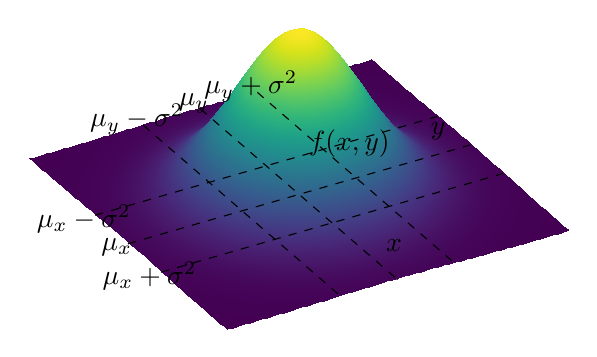
\begin{tikzpicture}
		% Internal numeric placeholders for plotting (used only for computation)
		\pgfmathsetmacro{\muenum}{0}       % placeholder for ??
		\pgfmathsetmacro{\muynum}{0}       % placeholder for ?_y
		\pgfmathsetmacro{\sigsqnum}{1.0}     % placeholder for ?� (? = 1, so wider Gaussian)
		\pgfmathsetmacro{\scaleFactor}{6.0}  % scaling factor for visualization
		
		\begin{axis}[
			view={60}{30},
			axis lines=center,
			xlabel={$x$},
			ylabel={$y$},
			zlabel={$f(x,y)$},
			domain=\muenum-3:\muenum+3,
			y domain=\muynum-3:\muynum+3,
			samples=61,
			samples y=61,
			colormap/viridis,
			unit vector ratio={1 1 3}, % exaggerate the z-direction relative to x and y
			zmin=0, zmax=0.5,
			xtick=\empty, ytick=\empty, ztick=\empty,
			clip=false
			]
			% Plot the scaled bivariate Gaussian surface:
			% scaled_f(x,y) = scaleFactor * f(x,y), where
			% f(x,y) = 1/(2??�) exp(-((x-??)�+(y-?_y)�)/(2?�))
			\addplot3[
			surf,
			shader=interp,
			mesh/ordering=x varies,
			every mesh/.append style={draw=black, line width=0.2pt}
			]
			{ \scaleFactor * (1/(2*pi*\sigsqnum)*exp(-(((x-\muenum)^2+(y-\muynum)^2)/(2*\sigsqnum))) ) };
			
			% Dashed lines on the base (z=0) to mark x positions:
			\draw[dashed] (axis cs:\muenum,\muynum-3,0) -- (axis cs:\muenum,\muynum+3,0);
			\draw[dashed] (axis cs:{\muenum-\sigsqnum},\muynum-3,0) -- (axis cs:{\muenum-\sigsqnum},\muynum+3,0);
			\draw[dashed] (axis cs:{\muenum+\sigsqnum},\muynum-3,0) -- (axis cs:{\muenum+\sigsqnum},\muynum+3,0);
			
			% Dashed lines on the base (z=0) to mark y positions:
			\draw[dashed] (axis cs:\muenum-3,\muynum,0) -- (axis cs:\muenum+3,\muynum,0);
			\draw[dashed] (axis cs:\muenum-3,{\muynum-\sigsqnum},0) -- (axis cs:\muenum+3,{\muynum-\sigsqnum},0);
			\draw[dashed] (axis cs:\muenum-3,{\muynum+\sigsqnum},0) -- (axis cs:\muenum+3,{\muynum+\sigsqnum},0);
			
			% Label the x positions with generic symbols:
			\node at (axis cs:\muenum,{\muynum-3.2},0) {$\mu_x$};
			\node at (axis cs:{\muenum-\sigsqnum},{\muynum-3.2},0) {$\mu_x-\sigma^2$};
			\node at (axis cs:{\muenum+\sigsqnum},{\muynum-3.2},0) {$\mu_x+\sigma^2$};
			
			% Label the y positions:
			\node at (axis cs:\muenum-3.2,\muynum,0) {$\mu_y$};
			\node at (axis cs:\muenum-3.2,{\muynum-\sigsqnum},0) {$\mu_y-\sigma^2$};
			\node at (axis cs:\muenum-3.2,{\muynum+\sigsqnum},0) {$\mu_y+\sigma^2$};
			
			% Place the formulas (2D and generic multivariate) in a node with a newline between them.
			\node[anchor=west, align=left] at (axis cs:3.2,-2,0.3) {%
			};
		\end{axis}
	\end{tikzpicture}

\vspace{1cm} % Add vertical space between the picture and the formula

\begin{align*}
	f(x,y) &= \frac{1}{2\pi\,\sigma^2}
	\exp\!\Bigl(-\frac{(x-\mu_x)^2+(y-\mu_y)^2}{2\,\sigma^2}\Bigr)\\
	&= f(\mathbf{x}) = \frac{1}{\sqrt{(2\pi)^n\,|\Sigma|}}\exp\!\Bigl(-\frac{1}{2}(\mathbf{x}-\boldsymbol{\mu})^T\Sigma^{-1}(\mathbf{x}-\boldsymbol{\mu})\Bigr)
\end{align*}

\end{document}
